\section{Flask Overview}
Flask adalah sebuah Micro Web Framework untuk Bahasa pemrograman Python, yang mana  mempermudah
seorang developer dalam membuat sebuah Aplikasi Website. Flask adalah Framework umum
yang bisa di aplikasikan untuk Project yang skalanya berbeda-beda. untuk sebuah 
instansi, hal itu dapat digunakan untuk aplikasi web yang kecil dalam cakupan jaringannya.
prinsip fundamentalnya sama, yang mana bisa dengan mudah dibuatkan projectnya dalam skala aplikasi
website seperti apa saja \cite{alemu2014rest}.
\section{Flask PUT}
Put adalah metode yang digunakan untuk memperbaharui sumber daya. Ini melakukan operasi pembaruan. 
Tidak seperti POST, hanya mengeksekusi untuk memperbaharui sumber daya. Dalam PUT kita sama saja dengan kita 
melakukan aktivitas update, yang berarti dimana ada file yang sudah dibuat atau sudah jadi akan kita perbahurui 
dengan file yang baru dengan menggunakan perintah PUT.

\section{flask}
pada web server menyediakan sebuah flask yang dimaksud oleh flask yaitu digunakan hanya untuk suatu pengembangan dan pengujian. dan web server kini juga pengembangan flask sudah  dapat dijalankan secara terprogram dengan menerapkan metode app.run (). versi command yang  berfungsi lebih lama dan tidak pula memiliki perintah flask requidred serveryang untuk memulai dengan menjalankan skrip pada utama aplikasi.

\section{methods dalam Flask}
Ada beberapa method dalam flask yang terdiri dari GET, PUT,POST dan DELETE. Dari methods-methods tersebut masing-masing fungsinya berbeda, terutama untuk PUT akan dijelaskan lebih detail. PUT adalah metode yang digunakan untuk memperbarui sumber daya dengan konten yang diunggah. Method ini sangat fleksibel karena bisa berinteraksi dengan beberapa bahasa pemrograman lainnya seperti bahasa pemrograman pyhton.
\section{Pengertian Flask}
HTTP mendefinisikan seperangkat metode permintaan untuk menunjukkan tindakan yang diinginkan yang akan dilakukan untuk sumber daya tertentu. Meskipun mereka juga bisa menjadi kata benda, metode permintaan ini kadang-kadang disebut sebagai verba HTTP. Masing-masing menerapkan semantik yang berbeda, namun beberapa fitur umum digunakan bersama oleh mereka: mis. Metode permintaan dapat berupa safe, idempotent, atau cacheable.
PUT
Metode PUT menggantikan semua representasi terkini dari sumber target dengan muatan permintaan.


\section{PUT}
Web Service dapat didefenisikan sebagai sistem yang dirancang untuk mendukung interaksi antara berbagai macam mesin-mesin pada suatu jaringan.Web service menyediakan beberapa methode yaitu contohnya pada  HTTP untuk melakukan aktivitas HTTP tentu saja menggunakan perintahnya yaitu seperti  GET, POST, PUT atau DELETE dan fungsi dari perintah methode PUT yaitu untuk mengupdate atau memperbarui sebuah data.
fungsi dari flask PUT sendiri bukan hanya mengganti data saja tapi
juga digunakan sebagai perintah yang melakukan
penggantian semua data yang ada dengan data yang di update, sehingga
data yang tersedia dalam keadaan baru dan tidak terjadi error.
Source CODE untuk perintah flask PUT ini sendiri terdapat pada gambar \ref{4PUT} 
itu adalah contoh method flask PUT pada Python.

\begin{figure}[ht]
    \centerline{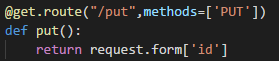
\includegraphics[width=1\textwidth]{figures/put.png}}
    \caption{Contoh Flask PUT method}
    \label{4PUT}
\end{figure}

\section{Perbedaan POST dan PUT}
POST dan PUT tentunya memiliki perbedaan secara arti maupun kegunaanya. POST yang berarti methode yang digunakan untuk pembuatan
instance baru dari sumber daya yang berarti merupakan operasi untuk membuat bukan memperbaharui data yang sudah ada. 
Sedangkan PUT merupakan methode yang digunakan untuk memberbaharui data yang sudah ada. Jadi POST itu untuk membuat 
sedangkan PUT untuk memperbaharui.